Die Topologie entspricht der vorgestellten Topologie und Rollenverteilung bzgl. der Infrastruktur (siehe Sektion \ref{sec: infra topologie}). Zusätzlich wird ein Back End in Form eines Servers benötigt, um den autonomen Verleih zu steuern.
\begin{figure}[H]
    \centering
    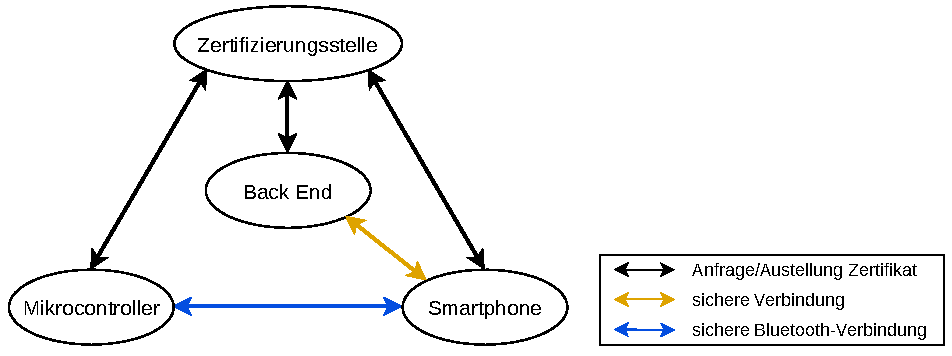
\includegraphics[width=1\textwidth]{graphics/impl_topologie.pdf}
    \caption[Topologie der Implementierung]{Topologie der Implementierung}
    \label{fig: impl topo}
\end{figure}
Abb. \ref{fig: impl topo} zeigt die Topologie der Implementierung. Bevor ein Ausleihprozess stattfinden kann, müssen Back End, Mikrocontroller und Smartphone jeweils über ein von der Zertifizierungsstelle ausgestelltes Zertifikat verfügen. Jeder Partei außer der Zertifizierungsstelle sollte periodisch (z.B. jährlich) ein Zertifikat ausgestellt werden.
\\\\
Innerhalb des Prototyps werden alle Zertifikate und privaten Schlüssel (auch das Root-Zertifikat und dessen privater Schlüssel) auf einem Personal Computer generiert. Beide Mikrocontroller erhalten beim "`Flashen"' des Programmes ein individuelles Zertifikat mit zugehörigem privaten Schlüssel.